The main variable to distinguish signals from and nuclear recoils, and
different types of background, is the energy density of the cluster.
To enhance the purity, a preselection is applied, prior to the tight
selection on $\delta$. Clusters with $p_l>500$ pixels, or $\xi<0.3$
are rejected, to remove the contribution from cosmic rays. A loose
selection on $\delta>5$ photons/pixel is applied, also to remove the
residual cosmic ray background based on their low specific ionization.
With this selection, the distribution in the 2D plane $\delta$--$l_p$
is shown in Fig.~\ref{fig:dvsl} for data with \ambe source, no source,
and the resulting background-subtracted \ambe data. The latter
distribution shows a component, present only in the data with \ambe
source, which has a moderate track length, $1.5<l_p<3.0$\unit{cm},
despite a much lower energy density than the one characteristic of the
energetic nuclear recoils ($9<\delta<12$). Since the density is
inversely proportional to the number of active pixels $n_p$, which is
correlated to the track length, the almost linear decrease of $\delta$
as a function of $l_p$ points toward a component with fixed
energy. The $^{241}$Am is expected to produce photons with
$E=59\keV$. This hypothesis is verified by introducing a diagonal
selection $\abs{\delta-y}<2$, where $y=14-p_l/50$, for the clusters
with $120<l_p<250$\unit{pixels}, which defines a control region
$PR$. The obtained energy spectrum for these clusters is shown in
Fig.~\ref{fig:59keV}, and indeed shows a peak at $E=65.6\pm3.2\keV$
(stat) for these photons, with the expected resolution. These events
are thus rejected by vetoing the $PR$ phase space.

\begin{figure}[ht]
  \begin{center}
  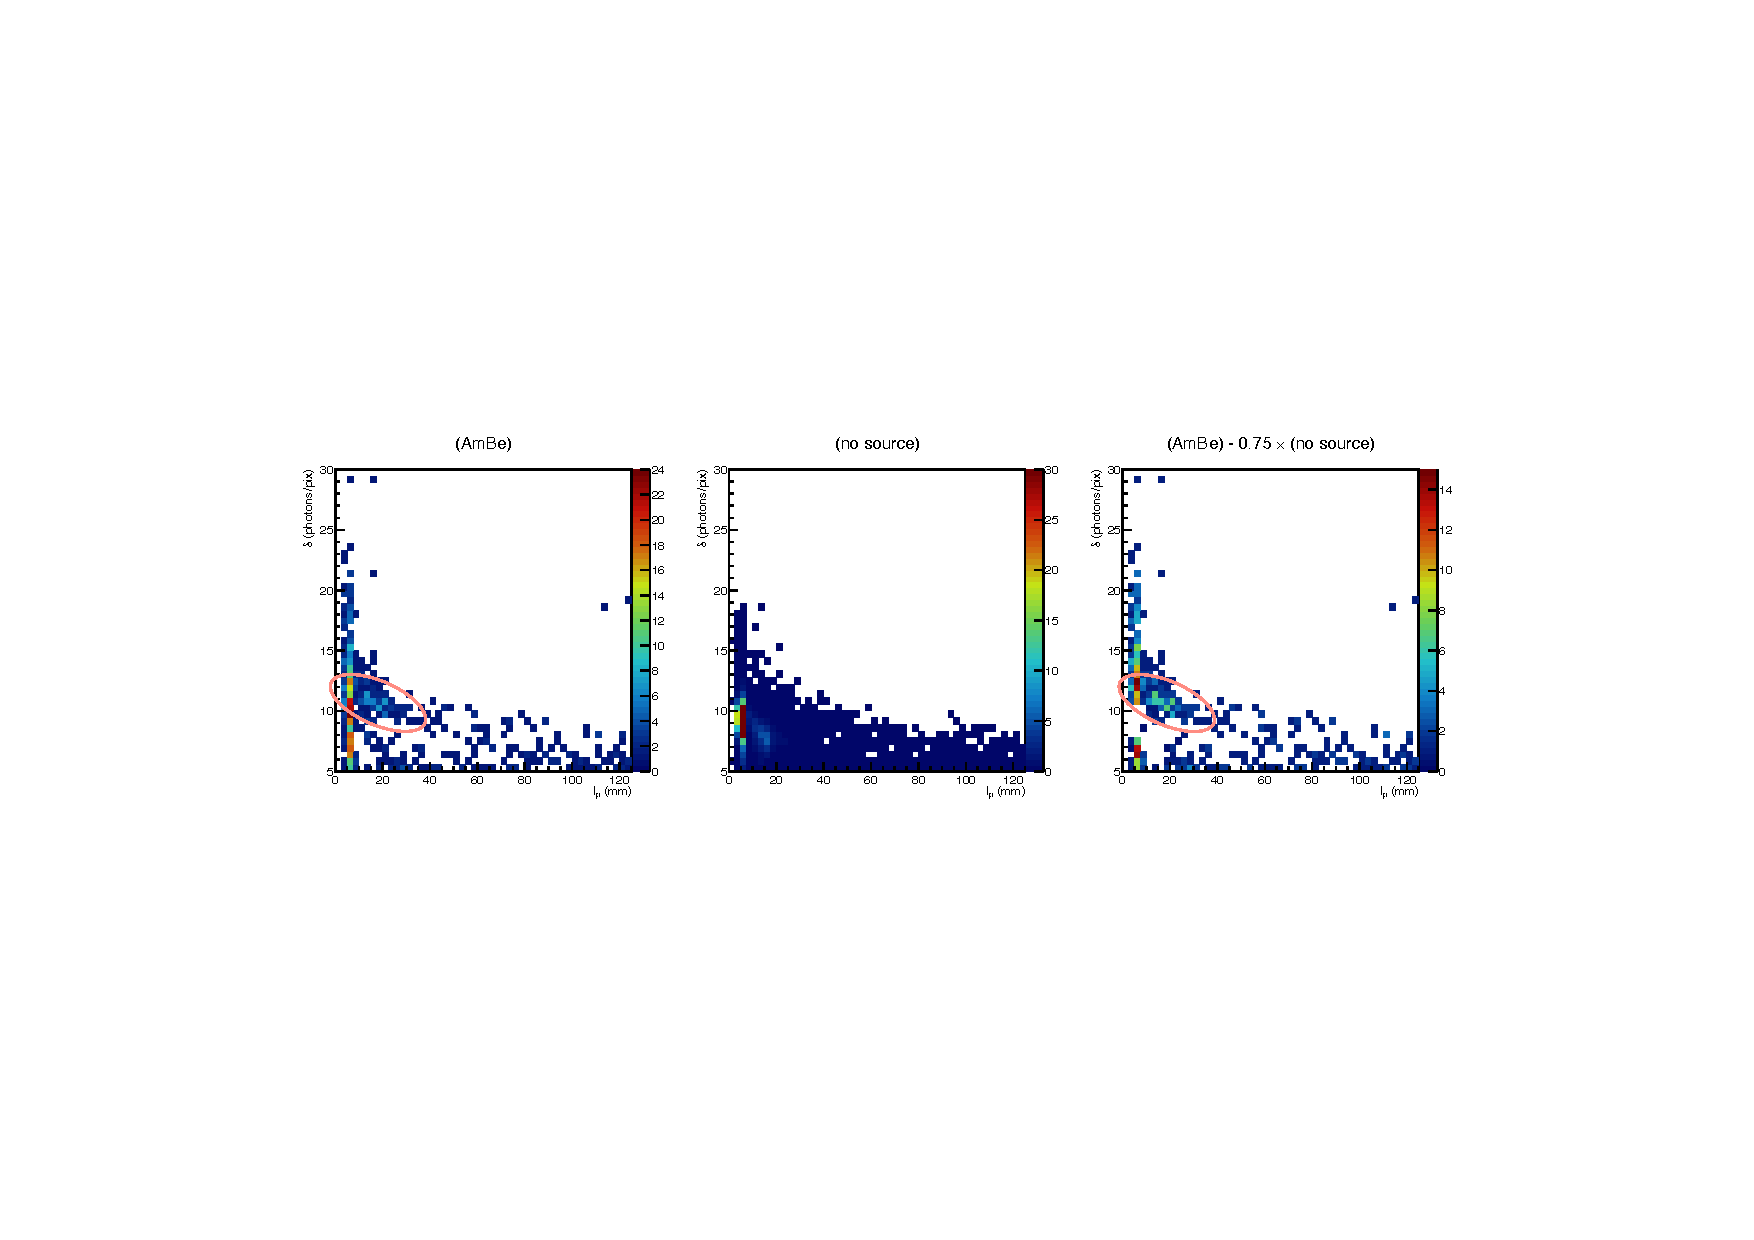
\includegraphics[width=0.90\linewidth]{figures/densityvslength_zoom}

  \caption{Supercluster light density $\delta$ versus length $l_p$,
    for data with \ambe source (left), data without any source
    (middle), and the resulting background-subtracted \ambe data.  The
    normalization of data without source is to the same exposure time
    of the \ambe one, accounting for the trigger scale factor
    $\varepsilon_{SF}$, as defined in the text. \label{fig:dvsl}}

  \end{center}
\end{figure}

\begin{figure}[ht]
  \begin{center}
  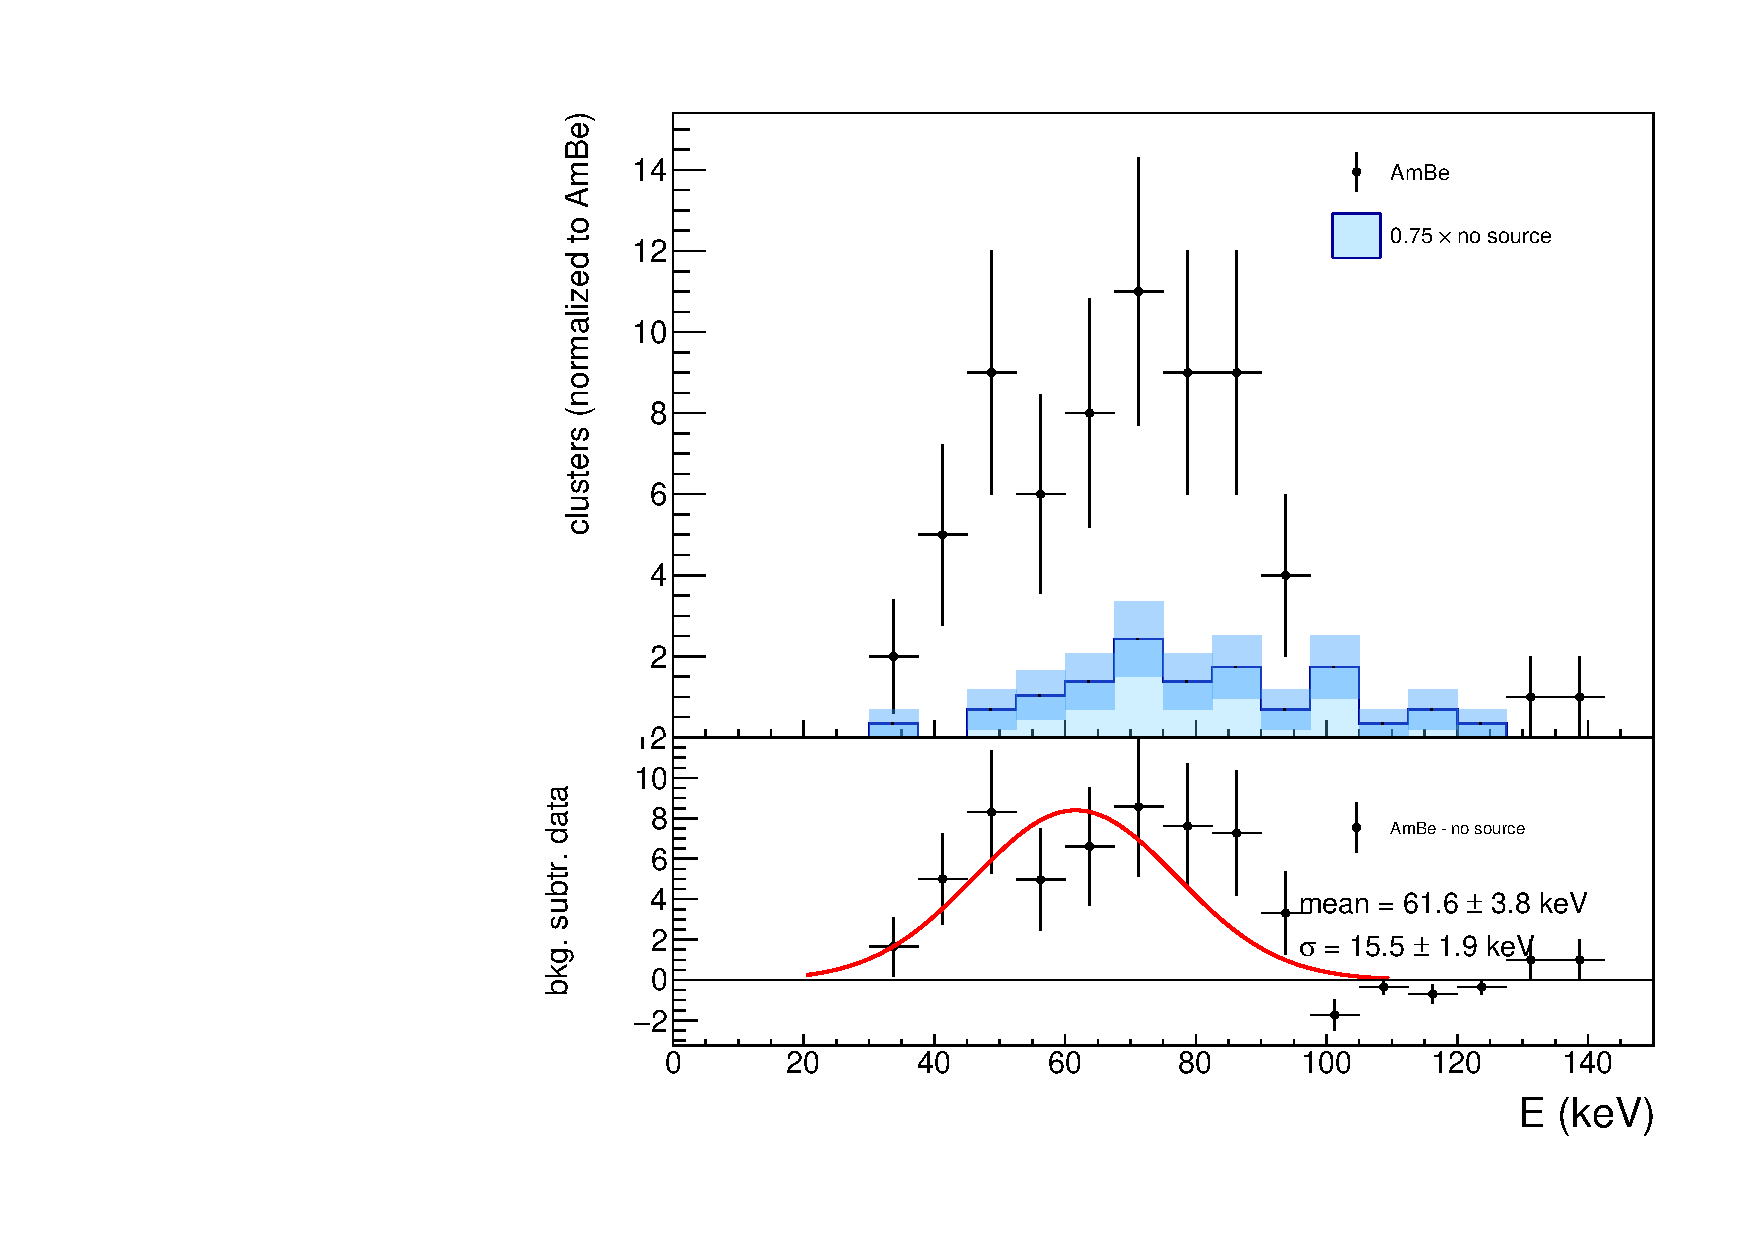
\includegraphics[width=0.60\linewidth]{figures/calintegral_59keV}

  \caption{Calibrated energy spectrum for candidates in the control
    region $PR$, as defined in the text. The background-subtracted
    distribution is fitted with a Gaussian PDF, which shows a mean
    value compatible with $E=59\keV$ expected from the $^{241}$Am
    $\gamma$s interacting with the gas. \label{fig:59keV}}

  \end{center}
\end{figure}

The light density, and the energy spectrum, after the full
preselection, is shown in Fig.~\ref{fig:presel}.
\begin{figure}[ht]
  \begin{center}
  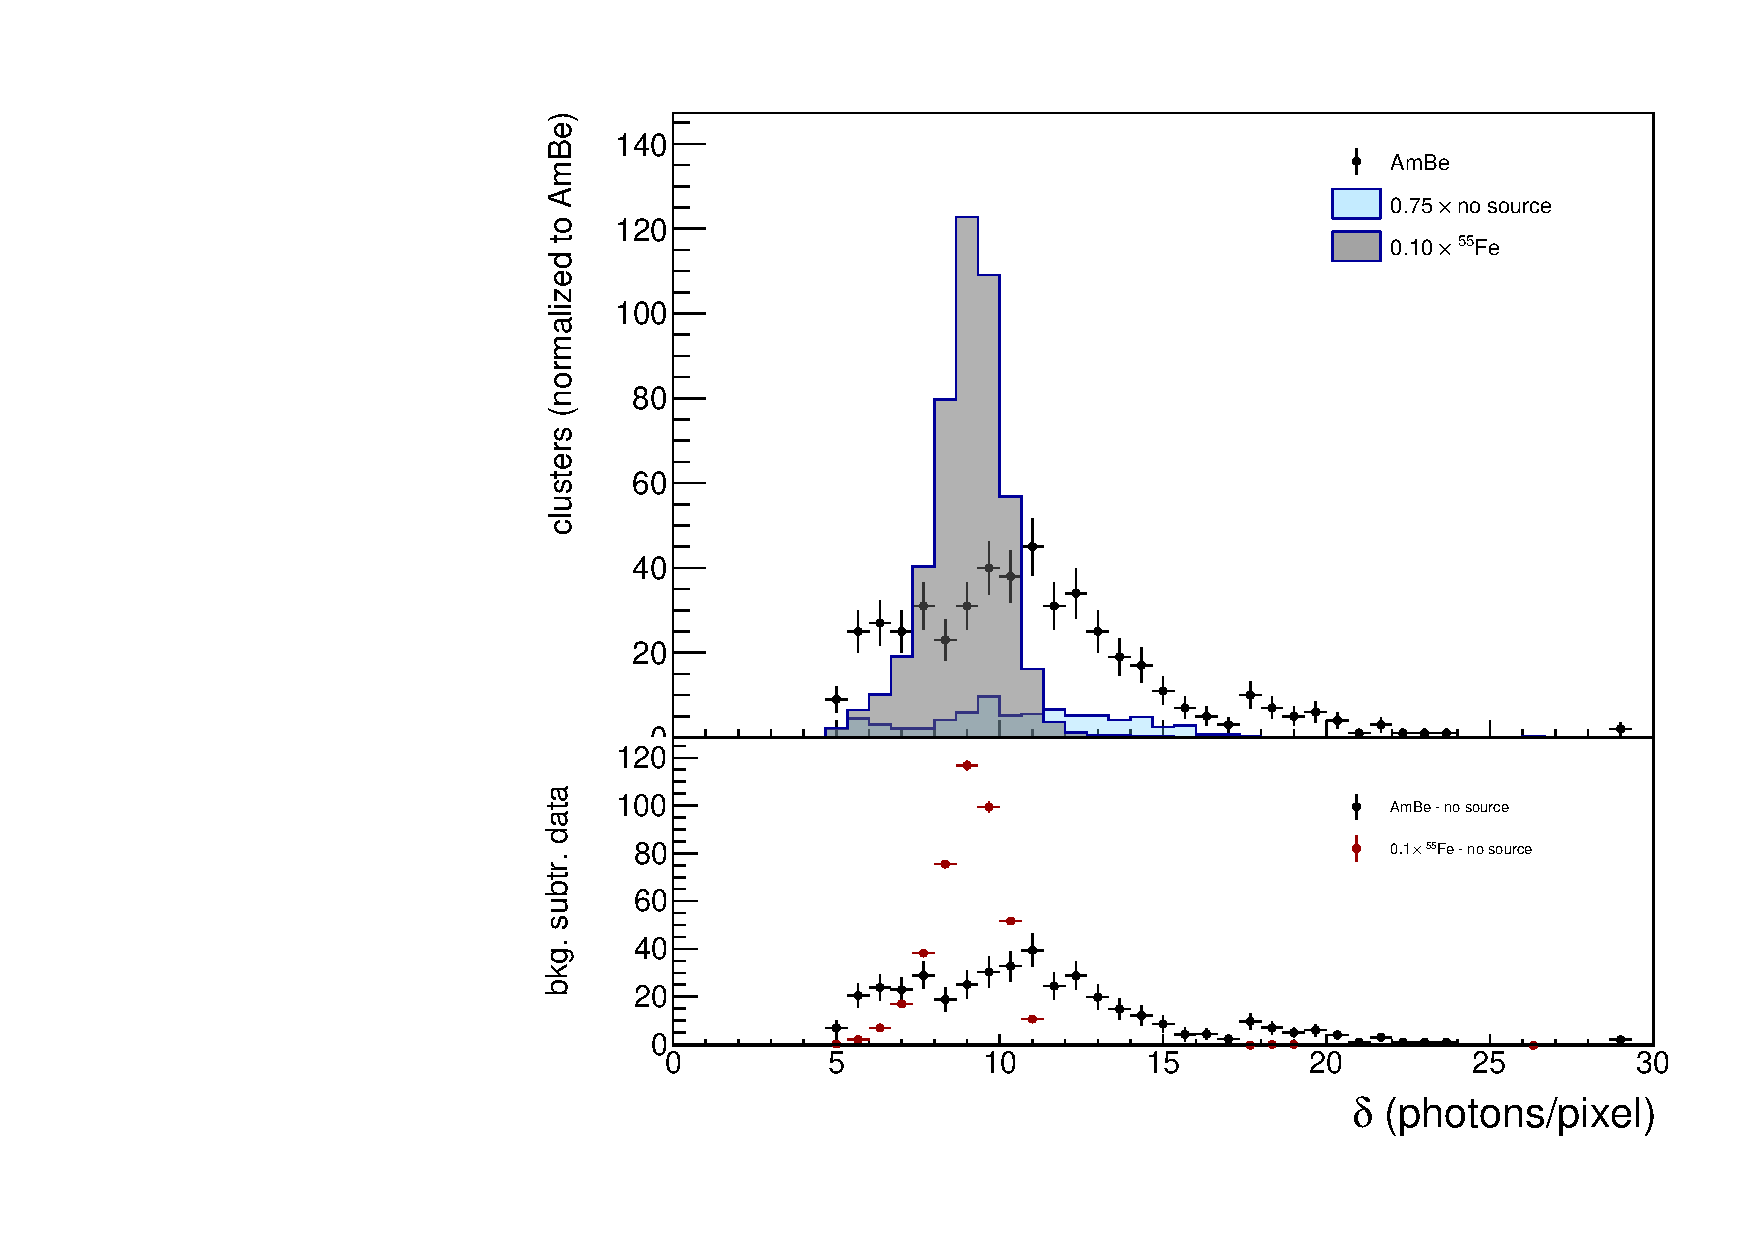
\includegraphics[width=0.45\linewidth]{figures/density_fullSel}
  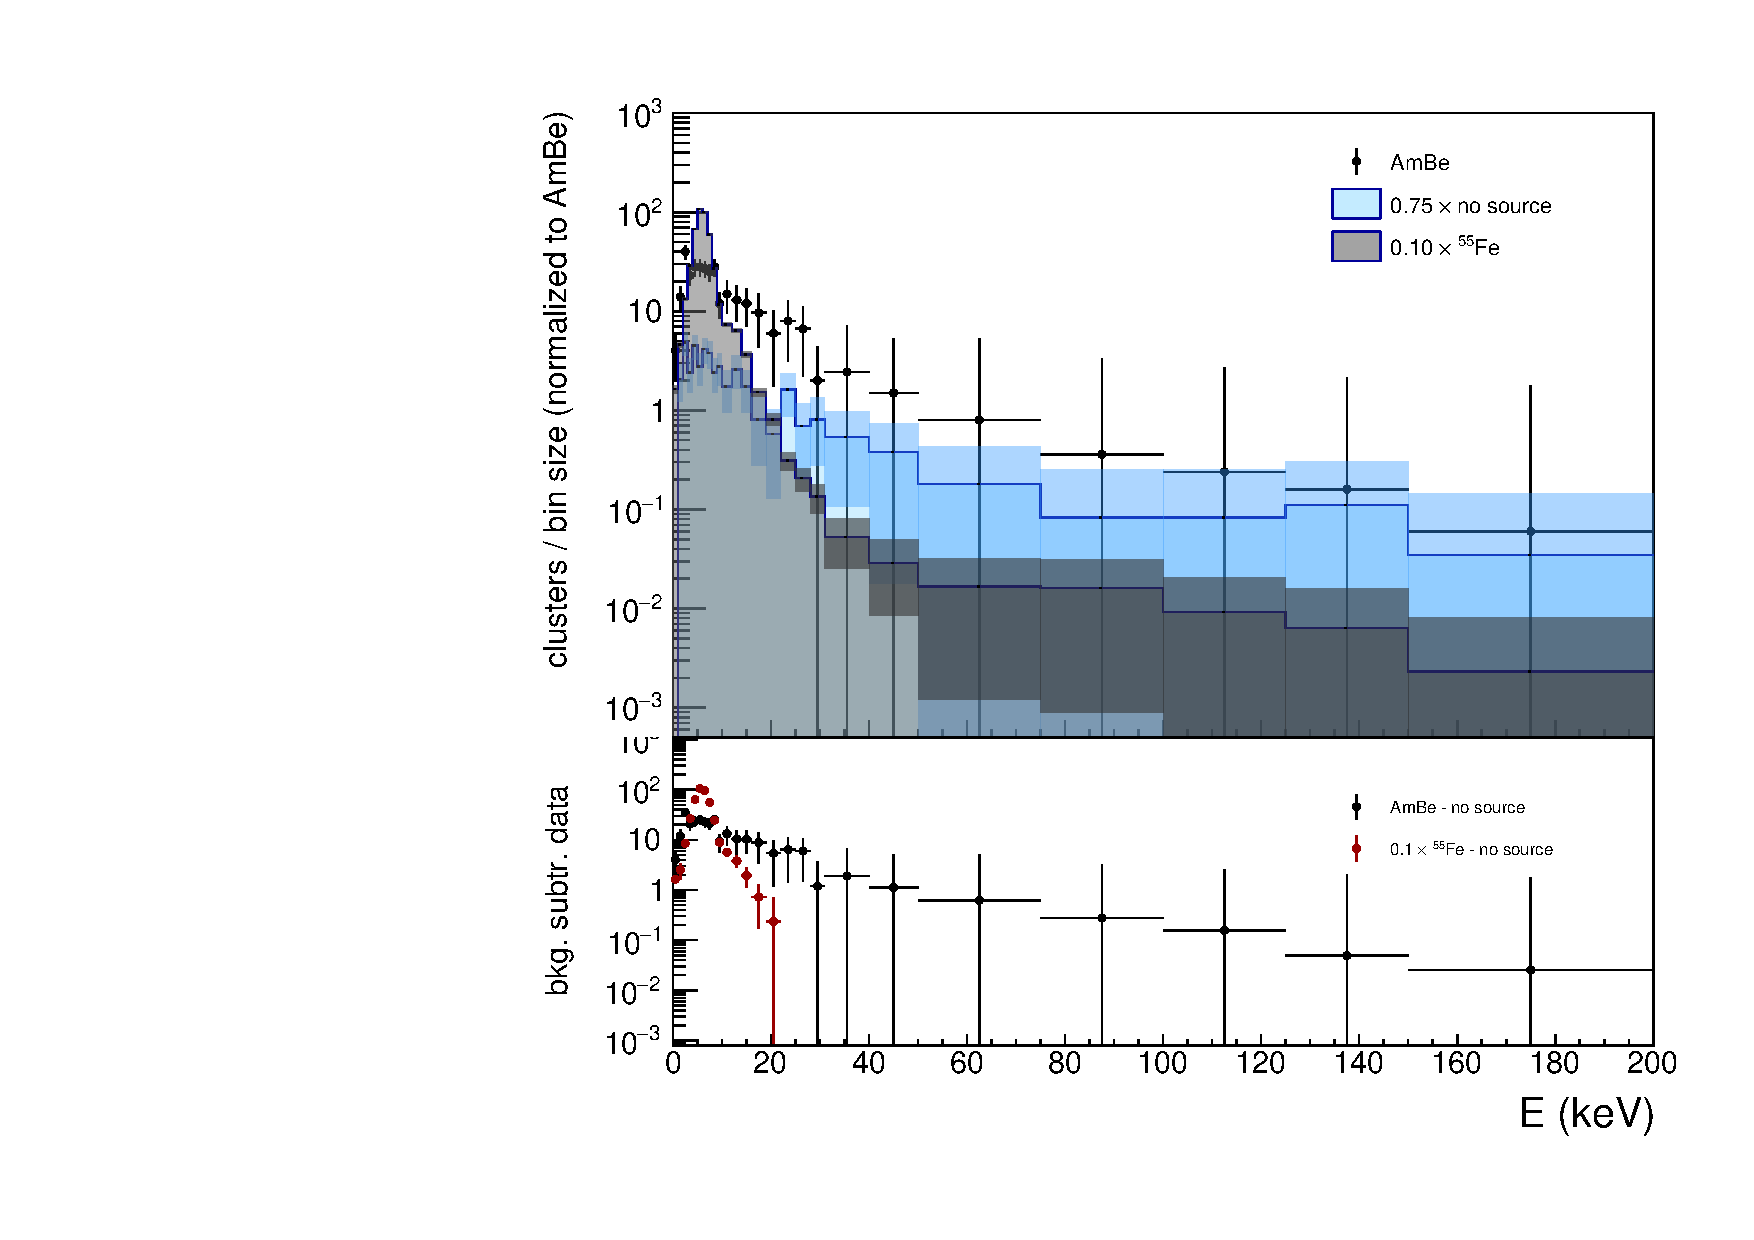
\includegraphics[width=0.45\linewidth]{figures/energy_fullSel}

  \caption{Supercluster light density $\delta$ (left) and calibrated
    energy (right), after the full preselection described in the text
    to select nuclear recoil candidates.  Filled points represent data
    with \ambe source, light blue distribution represents data without
    any source.  The normalization of data without source is to the
    same exposure time of the \ambe one, accounting for the trigger
    scale factor $\varepsilon_{SF}$, as defined in the text. For the
    data with \fe source, a scaling by a factor one tenth is applied
    for visibility, since the much larger cluster occupancy for these
    events.  \label{fig:presel}}

  \end{center}
\end{figure}

The light density, after the preselection, shows a large shape
difference between the data with \ambe source, data with \fe source,
and data without any source.  The background-subtracted distributions
of $\delta$ in \ambe data and \fe data, shown in bottom panels of
Fig.~\ref{fig:presel} (left), are used to evaluate a curve of electron
recoils rejection ($1-\varepsilon^\delta_{B}$) as a function of signal
efficiency ($\varepsilon^\delta_{S}$), obtained varying the selection on
$\delta$. This is shown in Fig.~\ref{fig:roc}. The same procedure
could be applied to estimate the rejection factor against the cosmic
ray induced background, but this is not shown because of the limited
sample without source and because this kind of background will be much
suppressed while operating a detector underground. This is shown in
Fig.~\ref{fig:roc}. While this cut-based approach is minimal, and
could be improved by profiting of the correlations among $\delta$ and
the variables used in the preselection in a multivariate analysis, it
shows that satisfying background rejections can be obtained, against
electron recoils from $E=6\keV$ photons.
%
\begin{figure}[ht]
  \begin{center}
  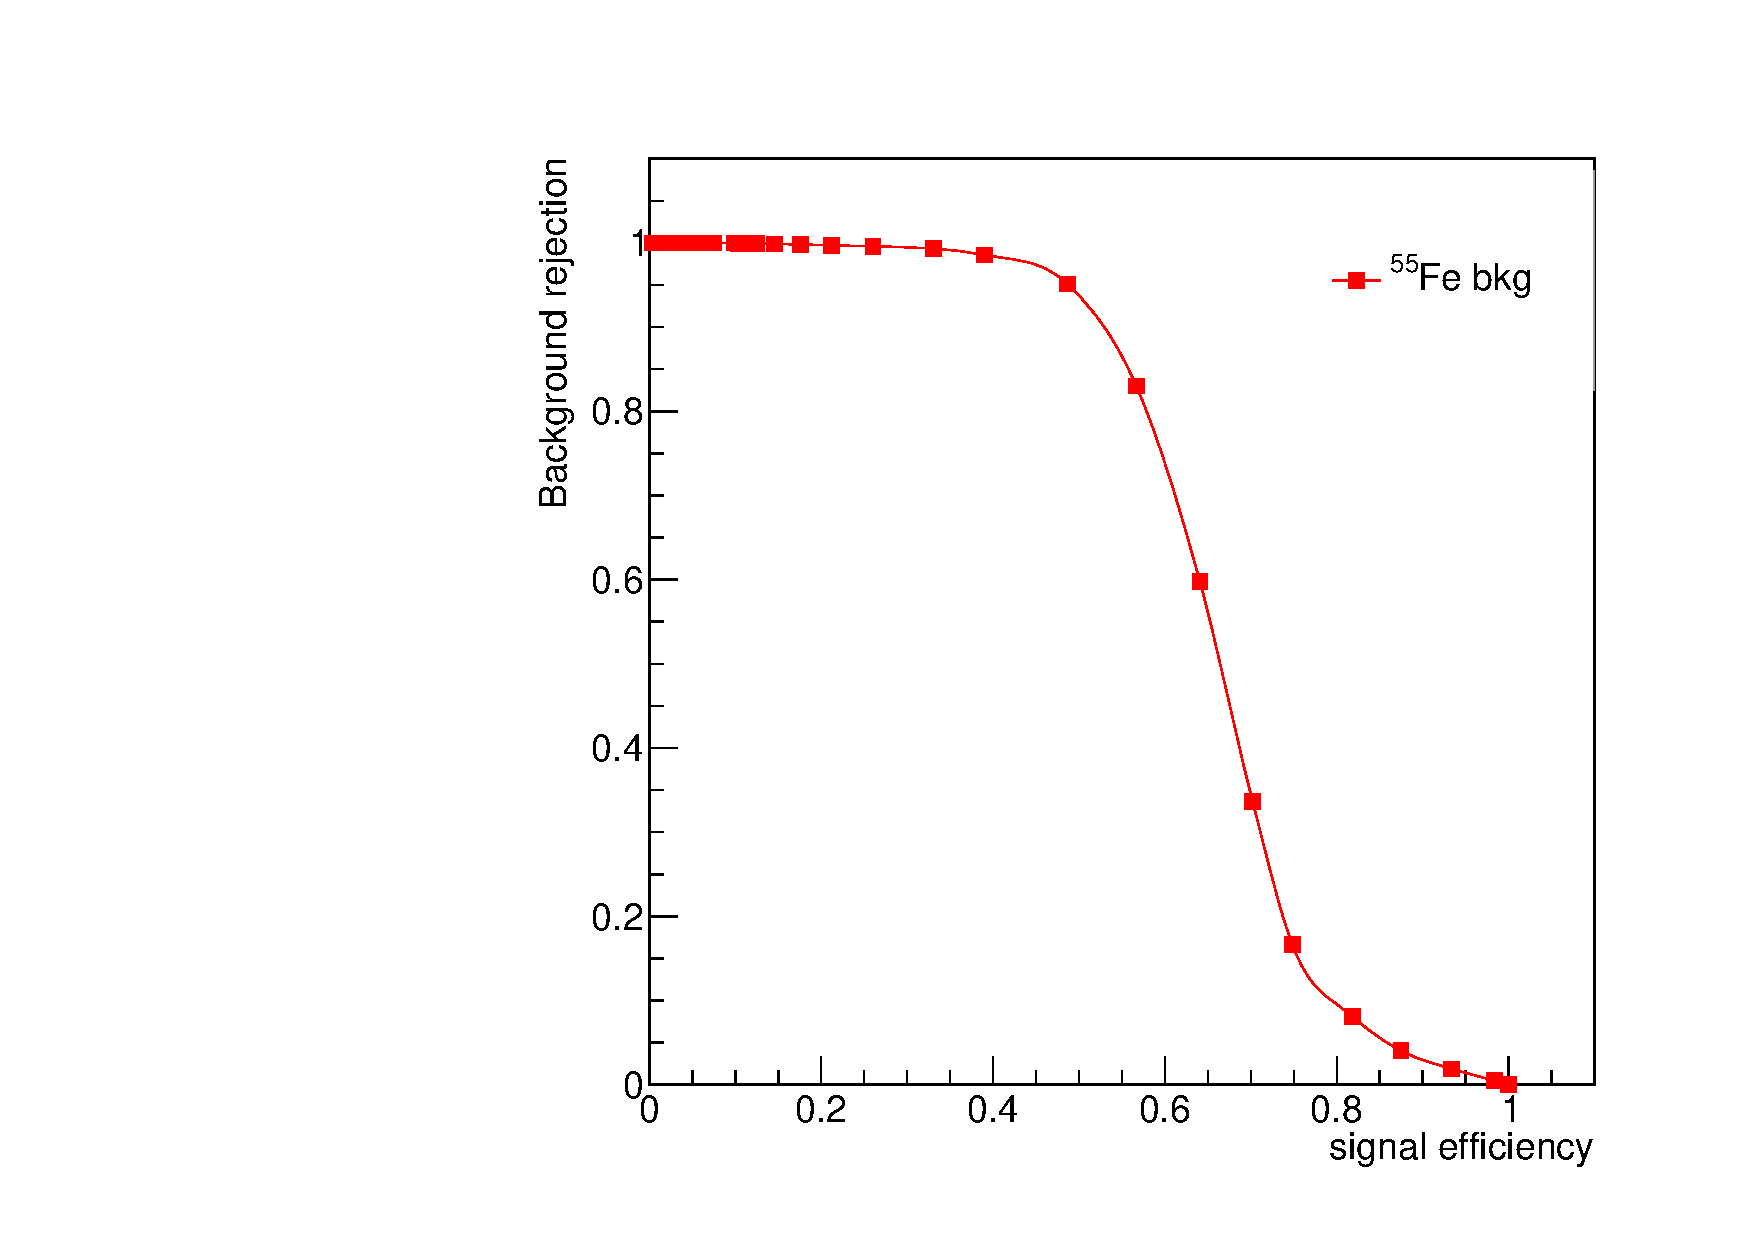
\includegraphics[width=0.45\linewidth]{figures/density_roc}

  \caption{Background rejection as a function of the signal
    efficiency, varying the selection on th $\delta$ variable in
    background-subtracted data with either \fe (background sample) or
    \ambe (signal sample) sources.  The $\delta$ distribution is the
    one obtained after the preselection described in the
    text.  \label{fig:roc}}

  \end{center}
\end{figure}
%

The efficiency of the preselection is assumed to be
$\varepsilon_{S}^{presel}=100\%$ on the signal, since it mostly
rejecting long tracks from cosmic rays. The efficiency of the
preselection on electron recoils is estimated on the \fe data sample,
and it is measured to be
$\varepsilon_{B}^{presel}=88\%$. Table~\ref{tab:roc} shows then the
full signal efficiency and electrons rejection factor for two example
working points, $\mathrm{WP}_{40}$ and $\mathrm{WP}_{50}$, having 40\%
and 50\% signal efficiency for the selection on $\delta$. They
correspond to a selection $\delta>11$ and $\delta>10$, respectively.


\begin{table*}[t]
\centering
\normalsize
\begin{tabular}{l c c c | c c c }
  \hline\hline
  working point & \multicolumn{3}{c}{Signal efficiency} & \multicolumn{3}{c}{Background efficiency} \\
  \hline
  & $\varepsilon_{S}^{presel}$ & $\varepsilon_{S}^{\delta}$ & $\varepsilon_{S}^{total}$ & $\varepsilon_{B}^{presel}$ & $\varepsilon_{B}^{\delta}$ & $\varepsilon_{B}^{total}$ \\
  \hline
  $\mathrm{WP}_{50}$  & 1                        & 0.5                      & 0.5                     & 0.88                     & 0.050                     & 0.040 \\
  $\mathrm{WP}_{40}$  & 1                        & 0.4                      & 0.4                     & 0.88                     & 0.012                     & 0.010 \\
  \hline\hline
\end{tabular}
\caption{Signal (nuclear recoils) and background (electron recoils) efficiency for
  two different selections on $\delta$.\label{tab:roc}}
\end{table*}

As an example, the energy spectrum for the candidates passing the
selection which is 50\% efficient on the \ambe sample is shown in
Fig.~\ref{fig:fullsel_effi} (left). With this selection, the signal
efficiency is computed for both the example working points in bins of
energy. The electron recoil efficiency, $\varepsilon_{B}^{total}$,
represents an overall background efficiency at a fixed energy
$E=6\keV$, characteristic of the \fe emitted photons.
%
\begin{figure}[ht]
  \begin{center}
    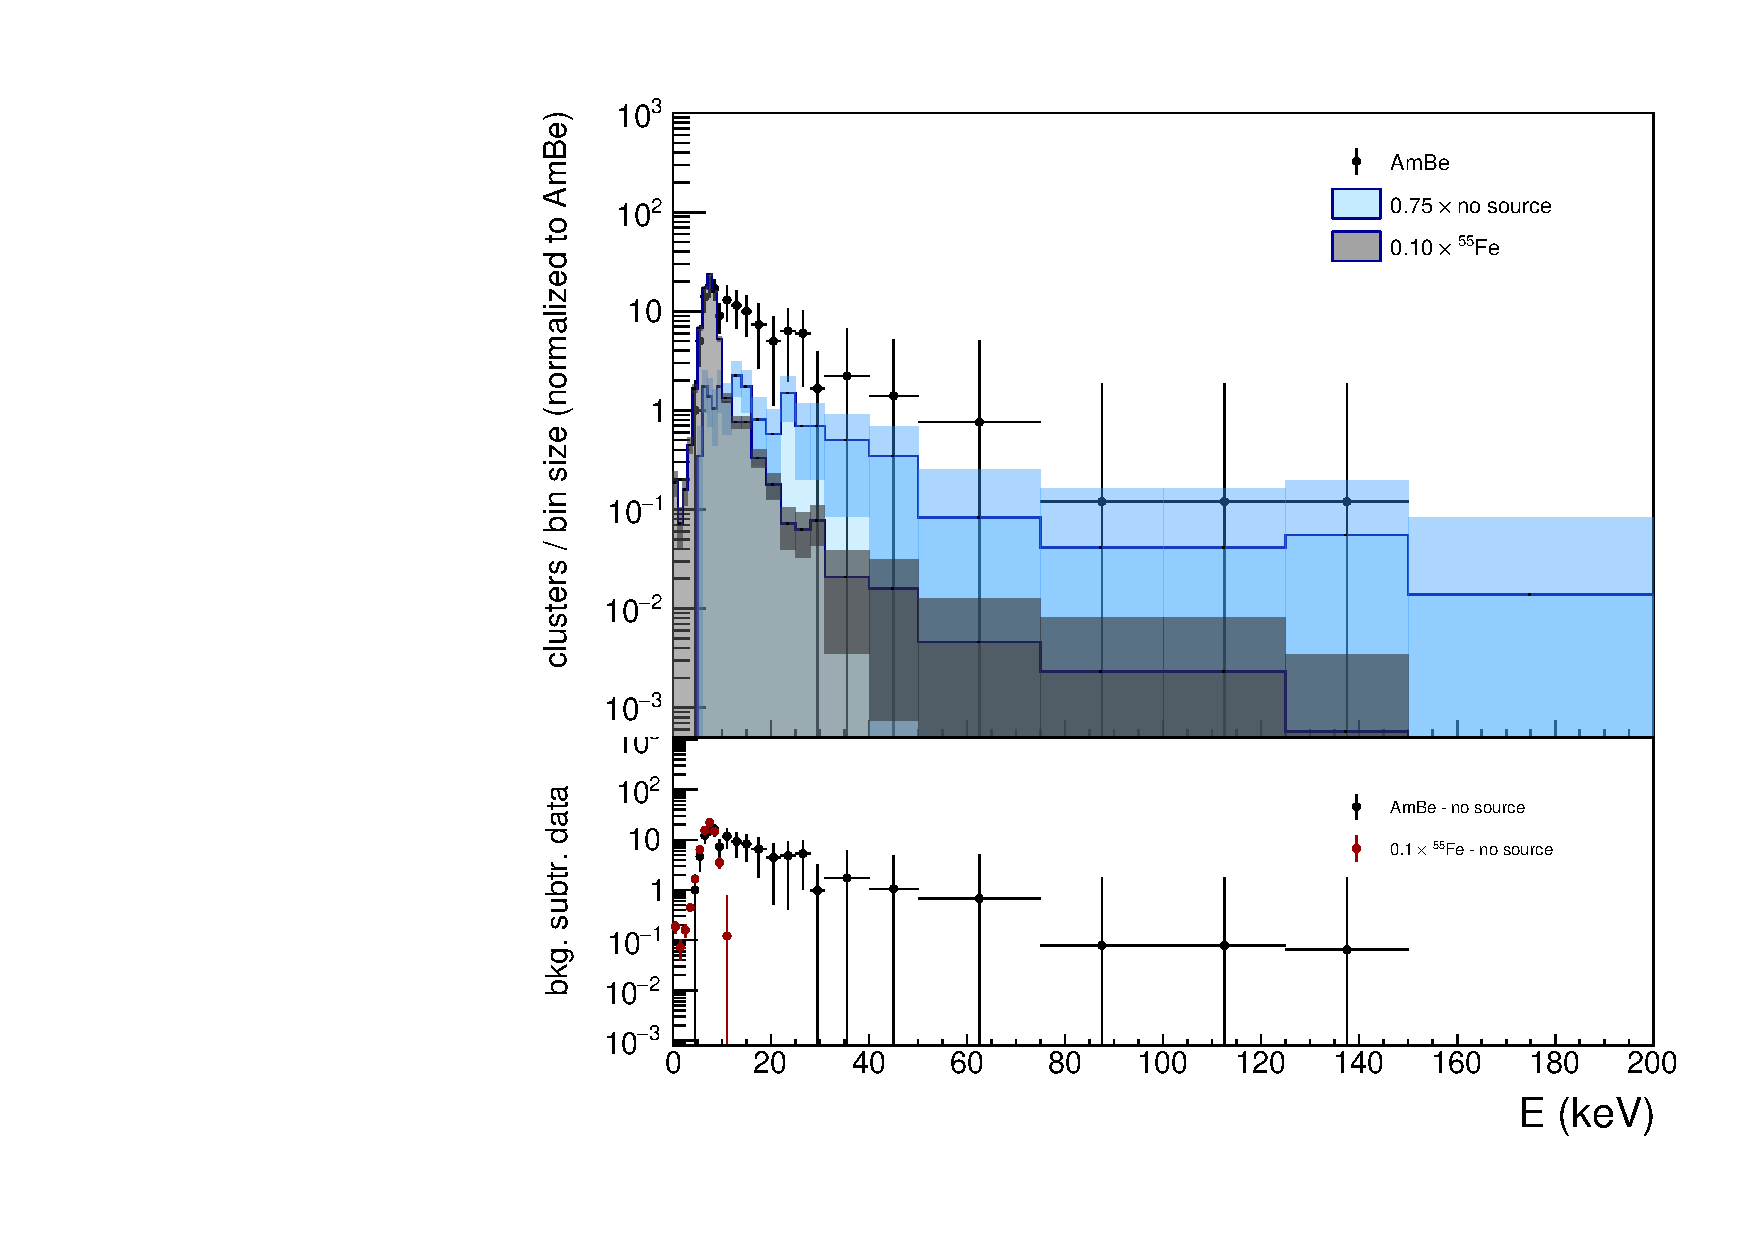
\includegraphics[width=0.45\linewidth]{figures/energyFull_WP50}
    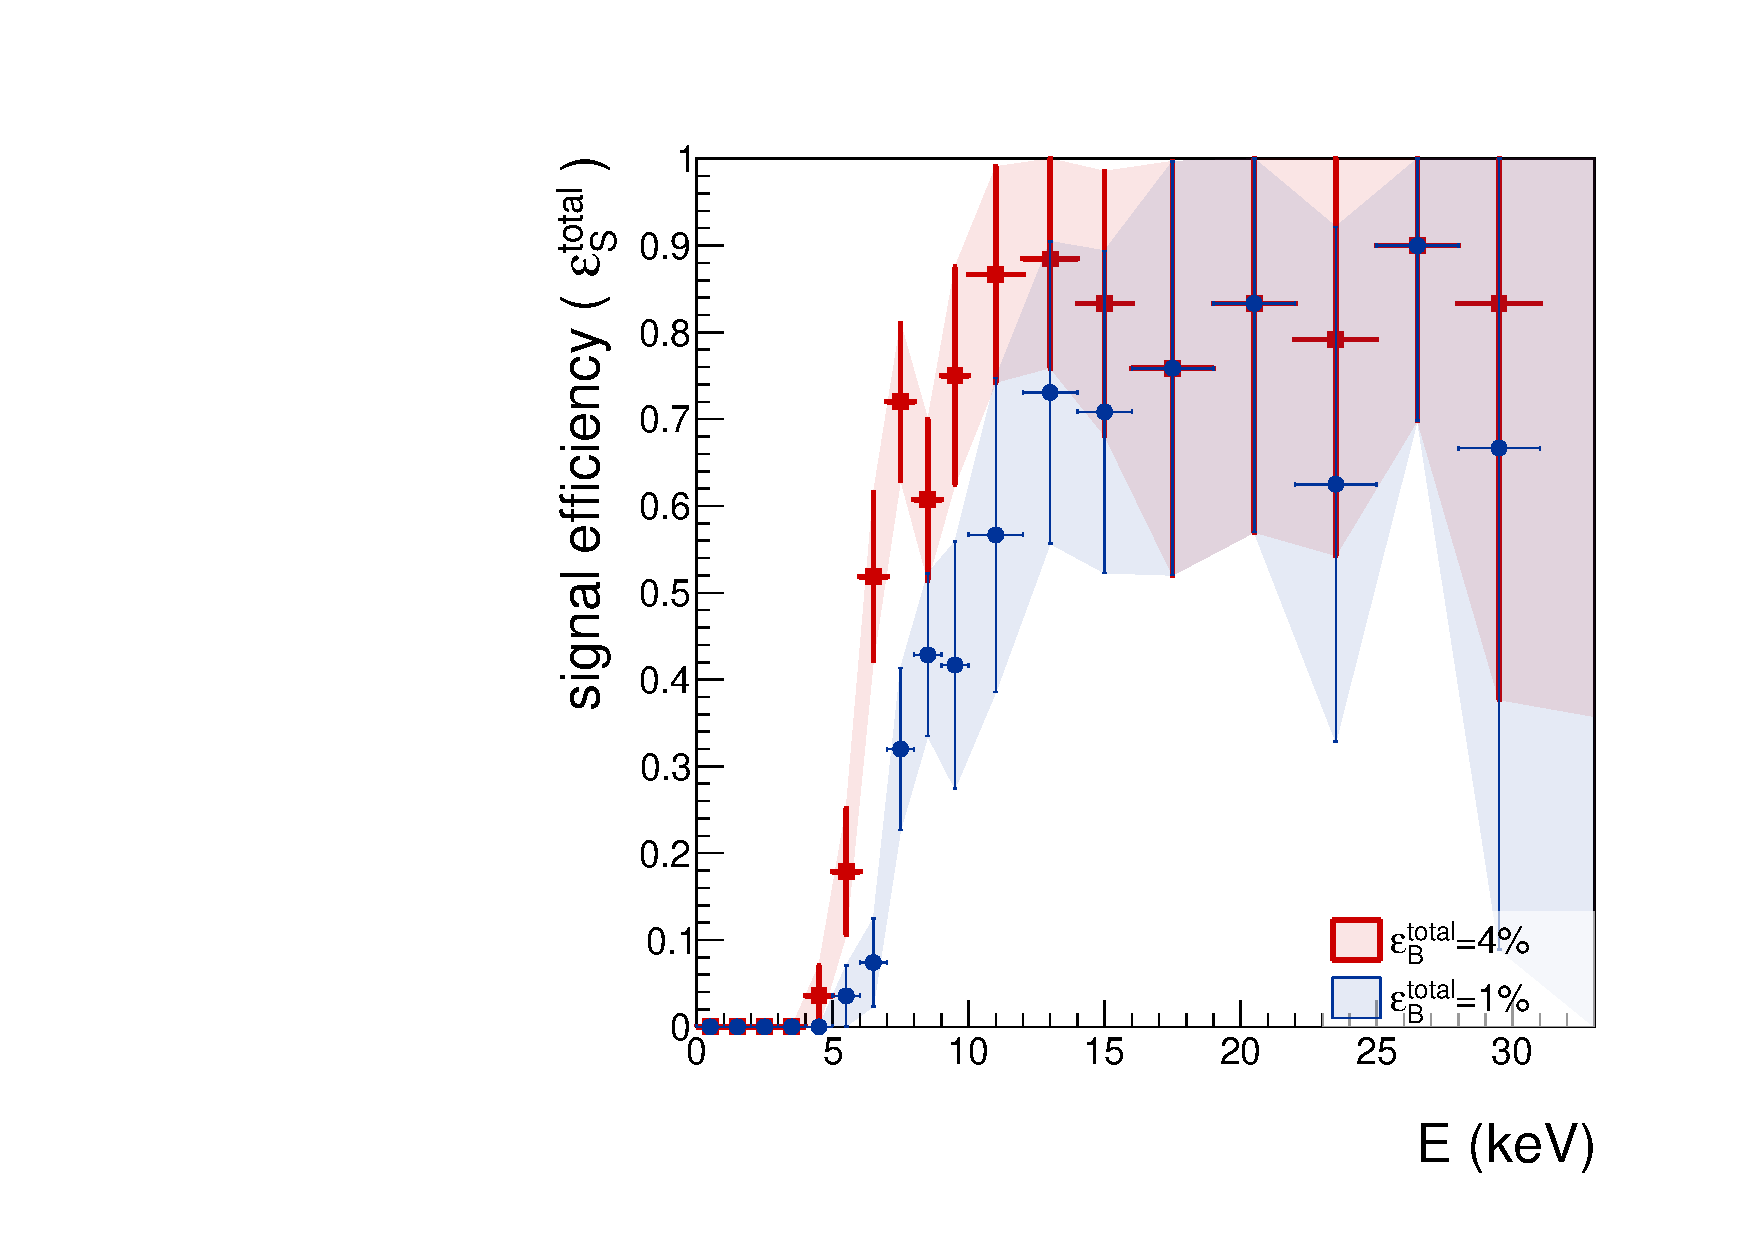
\includegraphics[width=0.45\linewidth]{figures/energyFull_effi}

    \caption{Left: supercluster calibrated energy (left), after the
      full selection, which includes $\delta>10$, 50\% efficient on
      signal, to select nuclear recoil candidates.  Filled points
      represent data with \ambe source, dark gray (light blue)
      distribution represents data with \fe source (no source).  The
      normalization of data without source is to the same exposure
      time of the \ambe one, accounting for the trigger scale factor
      $\varepsilon_{SF}$, as defined in the text. For the data with
      \fe source, a scaling by a factor one tenth is applied for
      visibility, since the much larger cluster occupancy for these
      events. Right: efficiency for nuclear recoil candidates,
      estimated on \ambe data, as a function of energy, for two
      example selections, described in the text, having either 4\% or
      1\% efficiency on electron recoils at
      $E=6\keV$. \label{fig:fullsel_effi}}

  \end{center}
\end{figure}
